% Technical note -- draft 2 (2026-09-24): reference-propeller sensitivity added
% (Eq. pconv, Table tab:ref, confronto_elica.py) and text corrections; draft 1 is
% nota_tecnica_bozza1.tex.
% Figures are read from ../out/. Compile with pdflatex (e.g. on Overleaf: upload this file
% and the PNG files of out/ into the same project, then remove the \graphicspath line).
% Items marked \todo{...} must be checked or filled in before submission.
\documentclass[11pt,a4paper]{article}
\usepackage[utf8]{inputenc}
\usepackage[T1]{fontenc}
\usepackage{amsmath,amssymb}
\usepackage{graphicx}
\usepackage{booktabs}
\usepackage{siunitx}
\usepackage[margin=2.5cm]{geometry}
\usepackage{xcolor}
\usepackage[hidelinks]{hyperref}
\graphicspath{{../out/}}
\newcommand{\todo}[1]{\textcolor{red}{[TODO: #1]}}
\newcommand{\ReV}{\mathit{Re}_V}
\newcommand{\ReL}{\mathit{Re}_L}

\title{Optimal streamlined bodies and the practical limits of tail-mounted\\
boundary-layer-ingesting propulsion: a reduced-order and RANS study}
\author{Pietro Buongiorno}
\date{\todo{date}}

\begin{document}
\maketitle

\begin{abstract}
We revisit two classical questions about bodies moving through a fluid at constant speed.
First, which axisymmetric shape minimises the drag at fixed volume or at fixed frontal area?
Second, how much propulsive power can be saved by placing the propulsor at the tail so that
it ingests the body's boundary layer (boundary-layer ingestion, BLI, as in the Goldschmied
body), and how large may the duct losses be before the saving disappears?
A two-dimensional lattice-Boltzmann model, an axisymmetric panel/integral-boundary-layer model
with shape optimisation, and axisymmetric RANS simulations ($k$--$\omega$ SST, OpenFOAM) are
combined. The optimum is a conventional elongated teardrop, with fineness ratio $L/D\approx3$
at fixed frontal area and $L/D\approx6$ at fixed volume; shapes based on the golden ratio or
golden spirals have 1.7--3.6 times the drag of the optimum (a sphere 7.5 times), in agreement
with Hoerner's classical data.
For a fully turbulent boundary layer the reduced-order model gives a break-even duct loss
$K^*$ that decreases from 8.5\% to 4.5\% of the free-stream dynamic pressure as $\ReV$ goes
from $3\times10^5$ to $10^8$. RANS simulations at $\ReV=10^6$ confirm the BLI gain: an
unducted actuator disc ingesting the boundary layer needs $8\%$ less power than the bare
body pushed by an ideal propeller of infinite disc area, and $15$--$18\%$ less than with an
isolated propeller of the same disc area. A flush wall slot loses essentially all the
ingested total pressure ($K\approx0.8$--$1.0$). A well-designed ducted intake with a rounded
lip keeps the intake loss at $K\approx2\%$, yet its self-propelled power ranges from $2\%$
below to $9\%$ above that of the conventional reference, depending on the size of the
reference propeller: the cowl skin friction, the altered afterbody pressure and the
acceleration of the ingested flow cancel most or all of the BLI benefit. The ideal BLI gain
and realistic installation penalties are of the same order, which explains the mixed
experimental record of Goldschmied-type bodies.
All codes and case generators are provided.
\end{abstract}

% ------------------------------------------------------------------
\section{Introduction}
Two questions motivate this note.
(i) Is there a ``special'' body shape --- for instance one based on the golden ratio or on a
logarithmic spiral --- that moves through a fluid with less resistance than the classical
streamlined body?
(ii) Can the propulsive power be reduced by re-energising the slow fluid of the body's own
boundary layer with a propulsor placed at the tail, instead of accelerating undisturbed
fluid with a conventional propeller?

The first question has a well-known answer in the engineering literature
\cite{hoerner1965}; we re-derive it with reproducible tools and quantify how far the
``golden'' shapes are from the optimum. The second question is the basis of the
Goldschmied body \cite{goldschmied1966} and of modern BLI aircraft concepts
\cite{smith1993,drela2009,dellacorte2022}. Its theoretical benefit is clear, but
experimental results for suction bodies have been contradictory \cite{roepke2012}. Our aim is to separate the ideal BLI gain from the installation losses
and to express the result as a simple design criterion: the maximum tolerable duct loss $K^*$.

% ------------------------------------------------------------------
\section{Methods}
\subsection{Two-dimensional lattice-Boltzmann screening}
A D2Q9 lattice-Boltzmann solver (\texttt{lbm.py}) was used at $Re=200$ (based on body
height $H$, 30 lattice units) to compare a circle, golden-ratio shapes (ellipse, rectangle,
teardrop, golden spiral) and teardrops of $L/H=3$ and $4.5$. A CMA-type evolution strategy
(\texttt{opt.py}) optimised a four-parameter shape at fixed area.

\subsection{Axisymmetric reduced-order model}
The inviscid flow is computed with an axisymmetric panel method; the boundary layer with an
integral method (laminar and turbulent closures, $e^N$ transition, separation detection)
(\texttt{axi.py}). Bodies are described by five parameters (fineness ratio and four shape
coefficients). The objective is the volumetric drag coefficient
$C_{D,V}=D/(\tfrac12\rho U^2V^{2/3})$ (fixed volume) or the drag based on frontal area.
Optimisation uses differential evolution (\texttt{axi\_opt.py}).

\subsection{BLI model and break-even loss}
The tail propulsor is modelled as an ingestion slot at $x_s$ with volume flow $Q$
(\texttt{bli.py}). The pump raises the total pressure of the ingested flow so that the
jet leaves at free-stream total pressure plus the momentum needed for self-propulsion.
Duct losses are expressed as a total-pressure loss $K\,\tfrac12\rho U^2$. The same blade
efficiency $\eta=0.85$ is used for the pump and for the reference propeller, so the
comparison isolates the BLI physics and the duct loss. For each $\ReV$ and $K\in\{0,0.05,
0.10,0.20\}$ the body shape, $x_s$ and $Q$ are optimised jointly (\texttt{bli\_opt.py},
\texttt{soglia.py}); $K^*$ is the loss at which BLI and conventional propulsion require the
same power.

\subsection{RANS simulations}
Axisymmetric RANS simulations were run with OpenFOAM 14 (\texttt{foamRun}, incompressible,
SIMPLEC, linear-upwind convection, $k$--$\omega$ SST \cite{menter1994}) on a
$5^\circ$ wedge (case generators \texttt{cfd\_caso.py}, \texttt{cfd\_blockmesh.py},
\texttt{cfd\_gold.py}, \texttt{cfd\_carena.py}). The body is the turbulent optimum at
$\ReV=10^6$ ($\ReL=4.95\times10^6$, $L/D=6.47$). Lengths are scaled by $L$, velocities by
$U$, forces are reported per wedge in units of $\rho U^2L^2$. The wall is resolved without wall functions: on the body the
area-averaged $y^+$ of the first cell is 0.32--0.43 and the maximum 0.54--0.89 in all cases;
on the cowl of the ducted case the average is 1.45 and the maximum 2.5.
The grid refinement of Sec.~\ref{sec:grid} increased the cell count in all directions but kept the
first-cell height, so $y^+$ is unchanged on the fine grids; a 5\% error on the cowl skin
friction would change the ducted power by about 0.8 points.

\emph{Inflow turbulence and tripping.} With low free-stream turbulence
($k=1.5\times10^{-6}$, $\omega=10$) the SST model stayed laminar over the whole body and
produced a spurious 45\% power saving. All cases reported here therefore use
$\omega_\infty=1.5$ ($\nu_t/\nu=5$) and a trip region ($k=0.005$, $\omega=100$ for
$0.03<x<0.08$). The eddy-viscosity distribution along the body was checked against the
bare-body reference in every case (\texttt{nut\_x.py}).

\emph{Propulsor.} The fan is an actuator disc (momentum source) of axial thickness $0.01L$.
Self-propulsion is reached iteratively: the disc thrust $T$ is set equal to the net drag of
body and cowl, the flow is re-converged, and the procedure is repeated three times
(\texttt{Allrun\_std}). The shaft power of an ideal disc is $P=T\,\langle u\rangle_{\rm
disc}$; it includes the kinetic energy left in the jet. It is compared with the bare body
pushed by an isolated (non-interacting) propeller in free stream, modelled as an actuator
disc of area $A_{\rm ref}$ with $T=D_{\rm bare}$:
\begin{equation}
P_{\rm conv}=D_{\rm bare}\,U\,\frac{1+\sqrt{1+C_T}}{2},\qquad
C_T=\frac{D_{\rm bare}}{\tfrac12\rho U^2A_{\rm ref}}.
\label{eq:pconv}
\end{equation}
with drag and area taken over the full annulus. The limit $A_{\rm ref}\to\infty$ gives $P_{\rm conv}=D_{\rm bare}U$ (ideal propeller, no jet
loss), the most favourable reference for conventional propulsion; unless stated otherwise,
power changes are quoted against this limit, and Table~\ref{tab:ref} gives the sensitivity to
$A_{\rm ref}$ (\texttt{confronto\_elica.py}).

\emph{Intake loss.} $K$ is the difference between the mass-averaged total pressure of the
captured stream tube at $x=0.835$ and at the fan face, divided by $\tfrac12\rho U^2$
(\texttt{misura\_K.py}, \texttt{misura\_carena.py}).

Configurations: (a) bare body; (b) free actuator disc at $0.895\le x\le0.905$, radius
$0.03$; (c) flush wall suction slot (Goldschmied type), slot widths $0.006$--$0.024$;
(d) ducted intake with an annular NACA-type cowl (leading edge at $x=0.855$, chord $0.095$,
thickness 5\%, mean radius $0.0293\to0.0249$; intake, fan and exit areas $2.54$, $1.91$,
$1.89\times10^{-3}\,L^2$) with the disc inside the duct.

% ------------------------------------------------------------------
\section{Results}
\subsection{Optimal body shape}
In 2D at $Re=200$ (Fig.~\ref{fig:lbm}) the area-based drag coefficient of the golden-ratio shapes is
$1.08$--$1.39$ (circle: $1.79$), against $0.73$ for the $L/H=3$ teardrop and $0.645$ for
the optimised shape ($L/H\approx8.3$) (Fig.~\ref{fig:opt}), and $0.566$ for the $L/H=4.5$
teardrop. The optimisation was run at a coarser resolution (body area 600 lattice cells,
$H\approx10$) than the comparison shapes ($H=30$), so its drag coefficient is not directly
comparable with the others; the 2D results are used only as a qualitative screening.
\todo{either repeat the 2D optimisation at $H=30$ or drop it}

In axisymmetric flow (Table~\ref{tab:shape}, Fig.~\ref{fig:opt3d}) the optimum at fixed
volume and turbulent boundary layer has $L/D=6.6$ ($\ReV=10^7$); with natural transition
$L/D=6.0$ at $\ReV=10^7$ and $9.3$ at $\ReV=10^6$ (long laminar run). At fixed frontal
area the optimum is $L/D=3.2$. Golden-ratio bodies ($L/D=1.618$) separate on the afterbody
and have 3--4 times the drag of the optimum; a sphere has about 7.5 times. These values are
consistent with Hoerner's compilation \cite{hoerner1965}.

\begin{table}[h]\centering
\caption{Axisymmetric shape optimisation (reduced-order model). $C$: drag coefficient on the
optimisation reference (volume$^{2/3}$ or frontal area).}\label{tab:shape}
\begin{tabular}{lcccccc}
\toprule
Case & $L/D_{\rm opt}$ & $C_{\rm opt}$ & golden ellipsoid & golden teardrop & sphere & $L/D=4.5$\\
\midrule
Volume, turbulent, $\ReV=10^7$ & 6.58 & 0.0172 & 0.0617 & 0.0530 & 0.1288 & 0.0175\\
Volume, natural, $\ReV=10^7$ & 6.00 & 0.0165 & 0.0609 & 0.0516 & 0.1279 & 0.0168\\
Volume, natural, $\ReV=10^6$ & 9.29 & 0.0072 & 0.0589 & 0.0540 & 0.1268 & 0.0133\\
Frontal area, turb., $Re_D=10^6$ & 3.17 & 0.0370 & 0.0967 & 0.0898 & 0.1400 & 0.0506\\
\bottomrule
\end{tabular}
\end{table}

\subsection{Break-even duct loss $K^*$}
For a fully turbulent boundary layer the ideal BLI saving ($K=0$) is 17--20\% of the power
of the optimal conventional body. The saving drops steeply with $K$
(Table~\ref{tab:kstar}, Fig.~\ref{fig:mappa}); the break-even loss $K^*$ decreases from
$8.5\%$ at $\ReV=3\times10^5$ to $4.5\%$ at $10^8$, because the boundary layer becomes
relatively thinner and carries less momentum deficit. At $\ReV=10^7$, three repeated
optimisations with different seeds and more iterations gave $K^*=5.83$, $5.85$ and $5.88\%$
(table value $5.77\%$), i.e.\ a spread of about $0.1$ percentage points; the repeatability
was not tested at the other Reynolds numbers.
The reference here is the ideal propeller ($P=D\,U/\eta$); the joint optimisation leaves the
ingested flow rate $Q$ free, so the BLI jet loss is also small. A finite-area reference
(Eq.~\ref{eq:pconv}) would raise $K^*$; the values in Table~\ref{tab:kstar} are therefore
conservative.
For natural transition the three transition criteria tested (Michel, $e^N$, Langtry--Menter
\cite{langtry2009}) give widely different laminar extents, and $K^*$ is not determined
reliably; we do not report it as a result (the shaded band in Fig.~\ref{fig:mappa} only shows
this spread).

\begin{table}[h]\centering
\caption{Power change of the BLI body relative to the optimal conventional body (turbulent
boundary layer), and break-even loss $K^*$.}\label{tab:kstar}
\begin{tabular}{rrrrrr}
\toprule
$\ReV$ & $K=0$ & $K=0.05$ & $K=0.10$ & $K=0.20$ & $K^*$\\
\midrule
$3\times10^5$ & $-20.1\%$ & $-6.5\%$ & $+2.9\%$ & $+15.9\%$ & 8.5\%\\
$10^6$ & $-19.8\%$ & $-4.8\%$ & $+4.7\%$ & $+18.1\%$ & 7.5\%\\
$3\times10^6$ & $-19.0\%$ & $-3.1\%$ & $+6.5\%$ & $+19.9\%$ & 6.6\%\\
$10^7$ & $-18.1\%$ & $-1.6\%$ & $+8.6\%$ & $+22.1\%$ & 5.8\%\\
$3\times10^7$ & $-17.3\%$ & $0.0\%$ & $+10.4\%$ & $+23.6\%$ & 5.0\%\\
$10^8$ & $-16.9\%$ & $+1.8\%$ & $+11.9\%$ & $+25.0\%$ & 4.5\%\\
\bottomrule
\end{tabular}
\end{table}

\emph{Validation against Goldschmied.} For Goldschmied's $L/D=3$ body at $\ReL=10^7$
($\ReV=3.7\times10^6$) the
model gives $C_{D,V}=0.0172$ with ideal suction against $0.0213$ for the best conventional
$L/D=3$ body ($-19\%$). Goldschmied reported $0.0162$ versus $0.0235$ for the Akron-type
reference ($-31\%$; $-26\%$ in total engine power) \cite{goldschmied1966}. The model therefore predicts a smaller, not a
larger, benefit than the original claim.

\subsection{RANS: bare body and free actuator disc}
The bare-body drag is $6.957\times10^{-6}$ per wedge, 4.6\% above the reduced-order model,
with matching pressure distribution (Fig.~\ref{fig:cfdconv}). With the free actuator disc
in self-propulsion, the ideal shaft power is $8.2\%$ lower than $P_{\rm conv}$ for an ideal
propeller, and $15.3\%$ lower than for an isolated propeller of the same disc area
($A=2.79\times10^{-3}L^2$, Table~\ref{tab:ref}). The disc
ingests the inner part of the boundary layer (mean axial velocity at the disc $0.89\,U$)
and the measured intake loss is $K\approx0\pm1\%$. This is the ideal BLI benefit at this
Reynolds number within RANS; $8.2\%$ is its lower bound.

\subsection{RANS: flush wall slot}
A flush suction slot gives $K\approx0.84$--$1.02$ for slot widths $0.006$--$0.012$ (and
$1.28$ for $0.024$). The no-slip wall condition across the slot removes the tangential
velocity of the ingested fluid: the slot behaves as a plenum intake that discards the
whole axial kinetic energy of the captured stream. Such an intake is far above $K^*$ and
cannot yield a net saving. (The slot cases were run with a prescribed jet velocity, not
in self-propulsion, on a different body (the natural-transition BLI optimum); their pump
power is therefore not reported as a power saving or penalty.) This is qualitatively
consistent with the Cal Poly wind-tunnel results \cite{roepke2012}.

\subsection{RANS: ducted intake with a rounded lip}
A first cowl design (intake area $3.4\times10^{-3}$, lip thickness 8\%) produced separation
and reversed flow ahead of the intake, with oscillating forces: the intake was too large
for the available boundary-layer flow. The final design (Sec.~2.4, case D) is attached
(Fig.~\ref{fig:carena}) and has $K=2.1\%$, well below $K^*$. Nevertheless the
self-propelled power is $9.2\%$ \emph{higher} than $P_{\rm conv}$ for an ideal propeller.
Against an isolated propeller of the same area as the fan ($A=1.94\times10^{-3}L^2$) it is
$2.1\%$ lower, and against a propeller as large as the free disc it is $0.9\%$ higher
(Table~\ref{tab:ref}). The ducted intake therefore gives no clear net gain.
Table~\ref{tab:budget} decomposes the difference relative to the bare-body drag.

\begin{table}[h]\centering
\caption{Force decomposition of the ducted configuration in self-propulsion, relative to
the bare-body drag $D_{\rm bare}=6.957\times10^{-6}$.}\label{tab:budget}
\begin{tabular}{lr}
\toprule
Cowl skin friction & $+15.4\%$\\
Lip suction (leading-edge thrust) & $-11.4\%$\\
Body drag increase (afterbody suction) & $+4.0\%$\\
\midrule
Required thrust $T/D_{\rm bare}$ & $1.080$\\
Mean axial velocity at the fan & $1.01\,U$ (free disc: $0.89\,U$)\\
Power $P/P_{\rm conv}$ (ideal propeller) & $1.092$\\
\bottomrule
\end{tabular}
\end{table}

\begin{table}[h]\centering
\caption{Self-propelled power of the BLI configurations relative to the bare body pushed by
an isolated propeller of disc area $A_{\rm ref}$ (Eq.~\ref{eq:pconv}; base grid). Fine grid,
equal-area references: free disc $-15.2\%$, ducted $-1.4\%$.}\label{tab:ref}
\begin{tabular}{lccc}
\toprule
Reference propeller & $A_{\rm ref}/L^2$ & Free disc & Ducted intake\\
\midrule
same area as the ducted fan & $1.94\times10^{-3}$ & $-17.8\%$ & $-2.1\%$\\
same area as the free disc & $2.79\times10^{-3}$ & $-15.3\%$ & $+0.9\%$\\
twice the free-disc area & $5.58\times10^{-3}$ & $-12.0\%$ & $+4.7\%$\\
half the body frontal area & $9.37\times10^{-3}$ & $-10.6\%$ & $+6.4\%$\\
body frontal area & $1.87\times10^{-2}$ & $-9.4\%$ & $+7.8\%$\\
infinite (ideal propeller) & $\infty$ & $-8.2\%$ & $+9.2\%$\\
\bottomrule
\end{tabular}
\end{table}
A fairer reference for the ducted intake would be an isolated ducted fan (nacelle) of the same
size, which also carries cowl friction; it has not been computed.

The duct accelerates the ingested flow to $1.01\,U$, so the fan no longer works on slow
fluid and the BLI benefit disappears. A simple estimate with the same cowl and a fan
velocity of $0.89\,U$ gives $P/P_{\rm conv}\approx0.96$ ($-4\%$ against the ideal
propeller); this has not been computed.

\subsection{Grid independence}\label{sec:grid}
On the refined grid the drag and the self-propelled powers change by less than one
percentage point, and the intake losses by at most 1.1 points (Table~\ref{tab:grid}). Two fine-grid runs (the ducted case with the standard inflow
settings, and the bare body with $\omega_\infty=0.3$ and a longer trip) converged instead
to a spurious laminar state: the eddy viscosity decayed along the body and, in the ducted
case, the laminar boundary layer separated at $0.54<x<0.70$. The SST solution is therefore
bistable and depends on the grid and on the initial conditions; these runs were discarded
after checking $\nu_t$ along the body. The fine ducted result reported here uses
$\omega_\infty=0.3$ and a trip extending to $x=0.15$; its $\nu_t$ distribution along the
body matches the base-grid case, and it is referred to the fine-grid bare body computed with
the standard settings. Self-propulsion was not fully converged (thrust and drag differ by
0.3\%); with $T=D$ the power change would be about $+9.7\%$.
\begin{table}[h]\centering
\caption{Grid sensitivity (refinement factor $\sqrt2$ per direction; powers against the
ideal propeller).}\label{tab:grid}
\begin{tabular}{lccc}
\toprule
Quantity & base grid & fine grid & change\\
\midrule
Bare-body drag ($\times10^{-6}$) & 6.957 & 6.969--6.973 & $+0.2\%$\\
Free disc: $P/P_{\rm conv}-1$ & $-8.2\%$ & $-8.1\%$ & 0.15 points\\
Free disc: $K$ & $0.5\%$ & $-0.6\%$ & 1.1 points\\
Ducted: $P/P_{\rm conv}-1$ & $+9.2\%$ & $+9.7$ to $+10.0\%$ & 0.5--0.8 points\\
Ducted: $K$ & $2.1\%$ & $2.0\%$ & 0.1 points\\
\bottomrule
\end{tabular}
\end{table}

% ------------------------------------------------------------------
\section{Discussion}
The ideal BLI benefit (8--18\% in RANS for this body depending on the reference propeller,
17--20\% in the reduced-order model, which optimises the shape jointly with the intake) is of
the same order as the losses of a realistic installation. The difficulty is intrinsic: for the fan to see slow
fluid the duct must diffuse, but a thick turbulent boundary layer that is further
decelerated separates ahead of the intake; if instead the duct accelerates the flow, the
intake is clean but the benefit is lost. The cowl itself adds wetted area whose friction is
comparable to the benefit. This explains why careful experiments on suction bodies have
struggled to reproduce the large savings originally reported.

\paragraph{Limitations.}
(1) Axisymmetric, steady RANS with a single turbulence model; no free-stream turbulence
effects beyond the trip. (2) Ideal actuator disc: no blade losses, swirl or
fan--distortion interaction. (3) A single cowl geometry was tested in RANS; the $-4\%$
estimate for a diffusing duct is not a computed result. (4) Laminar/transitional branch
unresolved. (5) One Reynolds number in RANS ($\ReV=10^6$). (6) The SST solution can fall into a
spurious laminar state (Sec.~\ref{sec:grid}); every result was screened for it, but the screening is
a posteriori. (7) The conventional reference is an isolated propeller that does not interact
with the body; the power changes depend on its assumed size (Table~\ref{tab:ref}).
(8) The grid study uses two grids with the same first-cell height; no third grid or
wall-resolution study was made. (9) The RANS results are compared with the reduced-order
model but not with independent experimental data.

\section{Conclusions}
\begin{enumerate}
\item The minimum-drag body is a conventional teardrop ($L/D\approx3$ at fixed frontal
area, $\approx6$ at fixed volume); golden-ratio shapes have 1.7--3.6 times the drag.
\item For turbulent boundary layers, tail BLI pays only if the duct loses less than
$K^*=4.5$--$8.5\%$ of the dynamic pressure (against an ideal propeller; a conservative
threshold).
\item A flush wall slot loses almost all the ingested total pressure and cannot pay.
\item An unducted tail propulsor ingesting the boundary layer saves 8--18\% of the power,
depending on the size of the conventional propeller it is compared with.
\item A clean ducted intake ($K=2\%$) is achievable, but cowl friction and flow
acceleration cancel most or all of the benefit (power between $-2\%$ and $+9\%$ of the
conventional reference). Recovering a clear net gain requires a duct that diffuses without
separating; this is the open design problem.
\end{enumerate}

\section*{Use of AI tools}
The codes, simulations, analysis and text of this note were developed with extensive
assistance from Claude (Anthropic), an AI assistant, under the direction of the author, who
checked the results and takes full responsibility for the content.

\section*{Code and data availability}
All scripts (Python 3, OpenFOAM 14), the exported RANS fields and the result files are
available at \url{https://github.com/buongiornopietro/tail-bli-propulsion}
(archived version: \todo{Zenodo DOI}). Table~\ref{tab:files} maps each figure and
table to the script that produces it; the repository README gives the commands.

\begin{table}[h]\centering
\caption{Scripts that produce each figure and table (all run from the repository root).}
\label{tab:files}
\begin{tabular}{ll}
\toprule
Item & Script (input $\rightarrow$ output)\\
\midrule
Fig.~\ref{fig:lbm} & \texttt{lbm.py} $\rightarrow$ \texttt{plot.py}\\
Fig.~\ref{fig:opt} & \texttt{opt.py} $\rightarrow$ \texttt{plot\_opt.py}\\
Table~\ref{tab:shape}, Fig.~\ref{fig:opt3d} & \texttt{axi.py}, \texttt{axi\_opt.py} $\rightarrow$ \texttt{plot\_axi.py}\\
Table~\ref{tab:kstar}, Fig.~\ref{fig:mappa} & \texttt{bli.py}, \texttt{bli\_opt.py}, \texttt{soglia.py} $\rightarrow$ \texttt{plot\_mappa\_finale.py}\\
Goldschmied validation & \texttt{valida\_goldschmied.py}\\
RANS cases & \texttt{cfd\_caso.py}, \texttt{cfd\_blockmesh.py}, \texttt{cfd\_gold.py}, \texttt{cfd\_carena.py}, \texttt{genera\_fini.py}\\
Fig.~\ref{fig:cfdconv} & \texttt{plot\_cfd.py}\\
Slot loss $K$ & \texttt{misura\_K.py}\\
Table~\ref{tab:budget}, Fig.~\ref{fig:carena} & \texttt{misura\_carena.py}, \texttt{plot\_carena.py}\\
Table~\ref{tab:ref} & \texttt{confronto\_elica.py}\\
Table~\ref{tab:grid} & \texttt{misura\_fine.py}\\
$\nu_t$ check along the body & \texttt{nut\_x.py}\\
\bottomrule
\end{tabular}
\end{table}

\begin{figure}[p]\centering
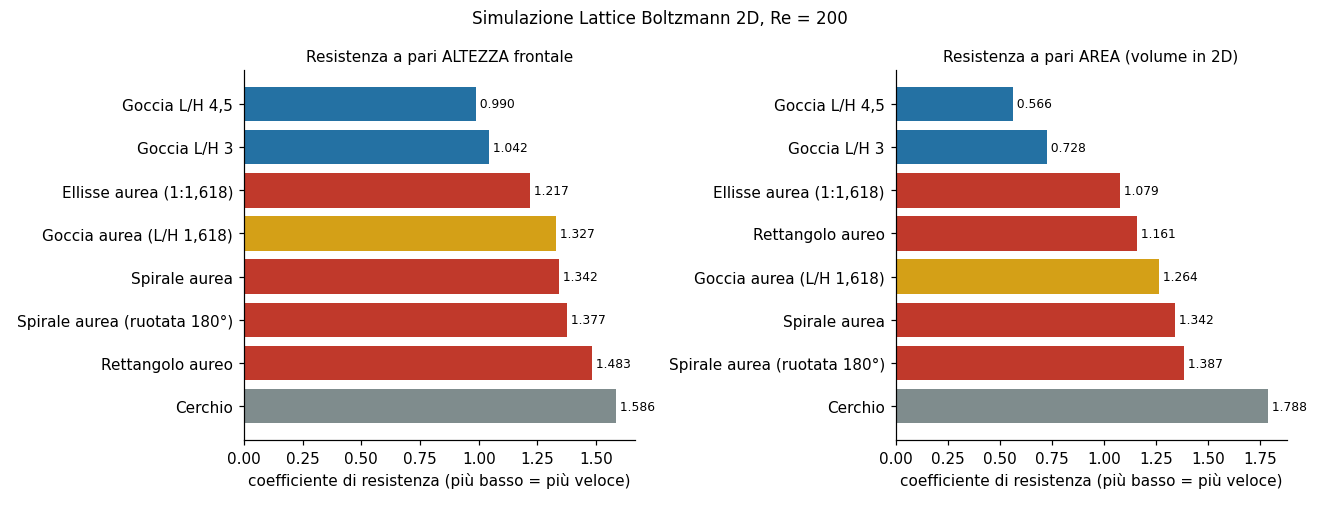
\includegraphics[width=0.8\linewidth]{resistenza_Re200.png}
\caption{2D lattice-Boltzmann drag at $Re=200$ for golden-ratio shapes and teardrops.}
\label{fig:lbm}
\end{figure}
\begin{figure}[p]\centering
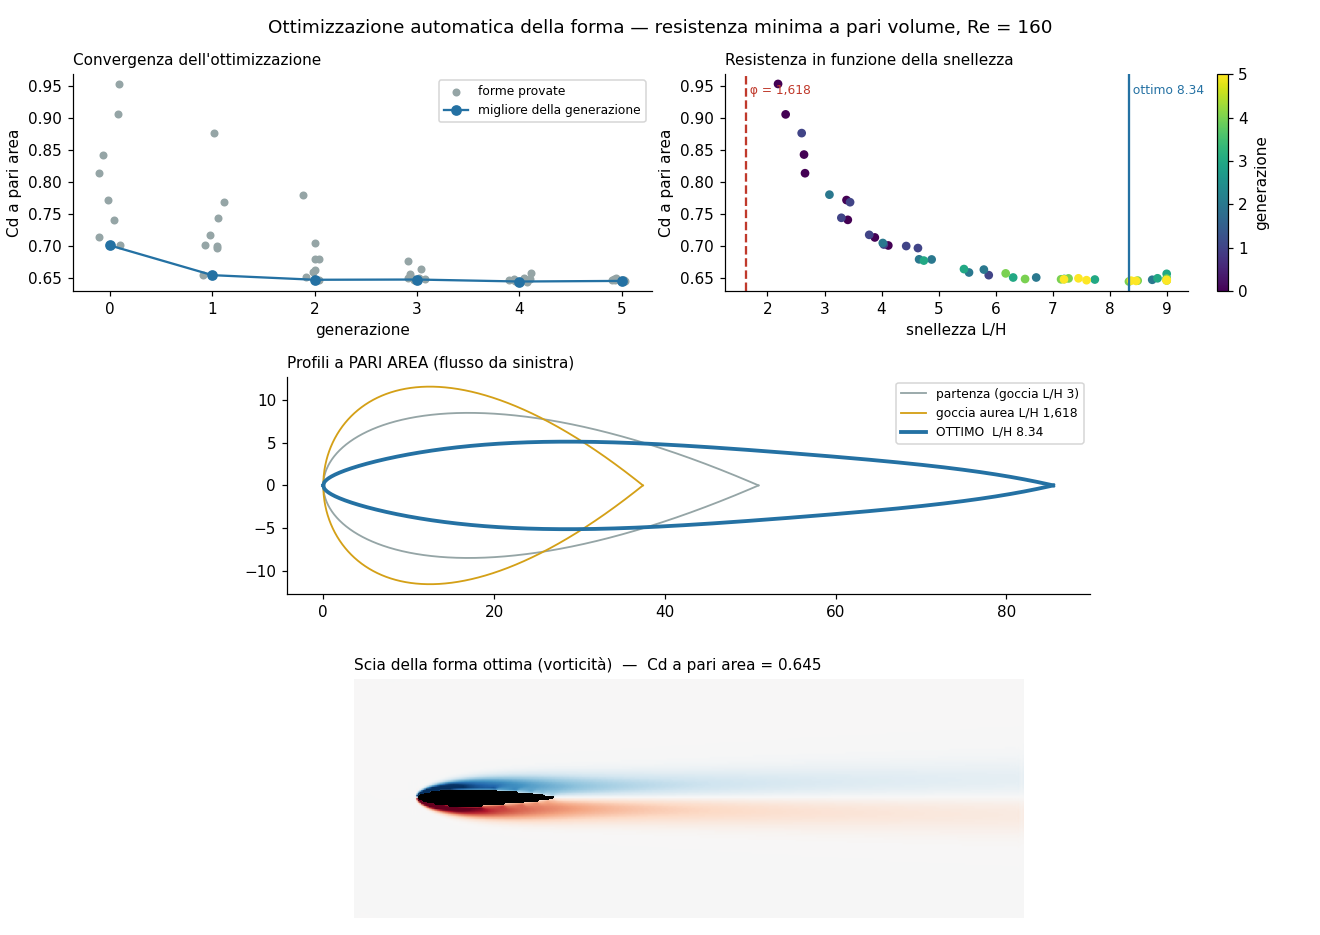
\includegraphics[width=0.8\linewidth]{ottimizzazione.png}
\caption{2D shape optimisation history.}\label{fig:opt}
\end{figure}
\begin{figure}[p]\centering
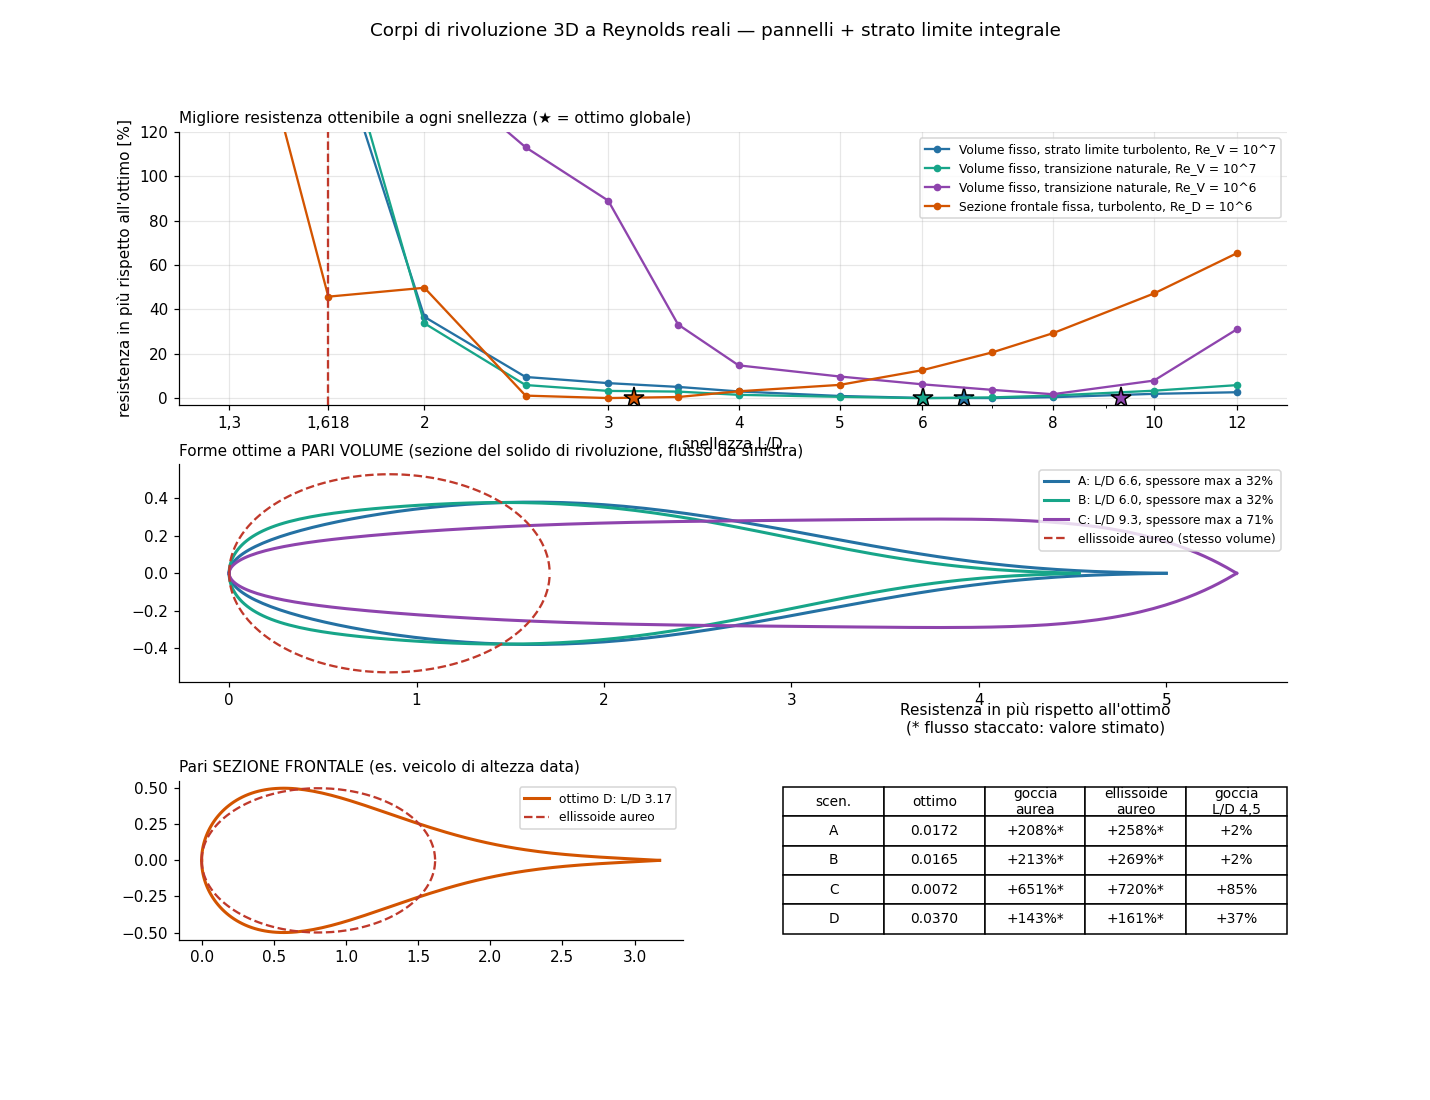
\includegraphics[width=0.8\linewidth]{ottimo_3D.png}
\caption{Axisymmetric optimal bodies.}\label{fig:opt3d}
\end{figure}
\begin{figure}[p]\centering
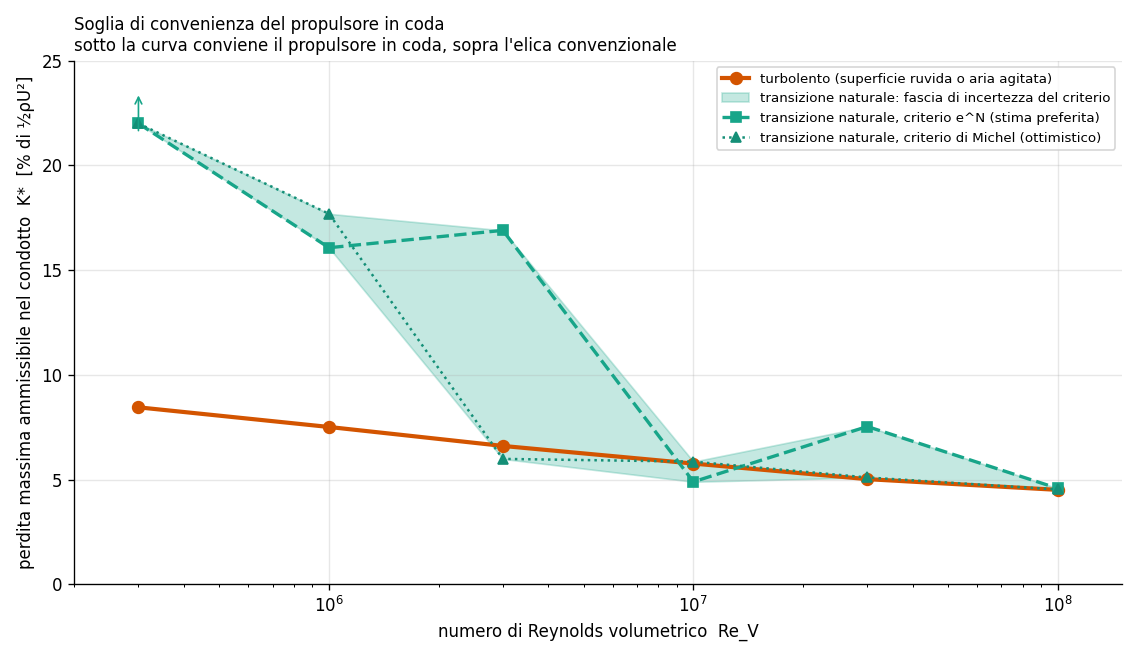
\includegraphics[width=0.8\linewidth]{mappa_finale.png}
\caption{Break-even duct loss $K^*$ versus $\ReV$. Solid line: fully turbulent boundary
layer (result). Shaded band: spread between transition criteria for natural transition,
shown for information only (not a result). \todo{figure labels to be translated into
English}}\label{fig:mappa}
\end{figure}
\begin{figure}[p]\centering
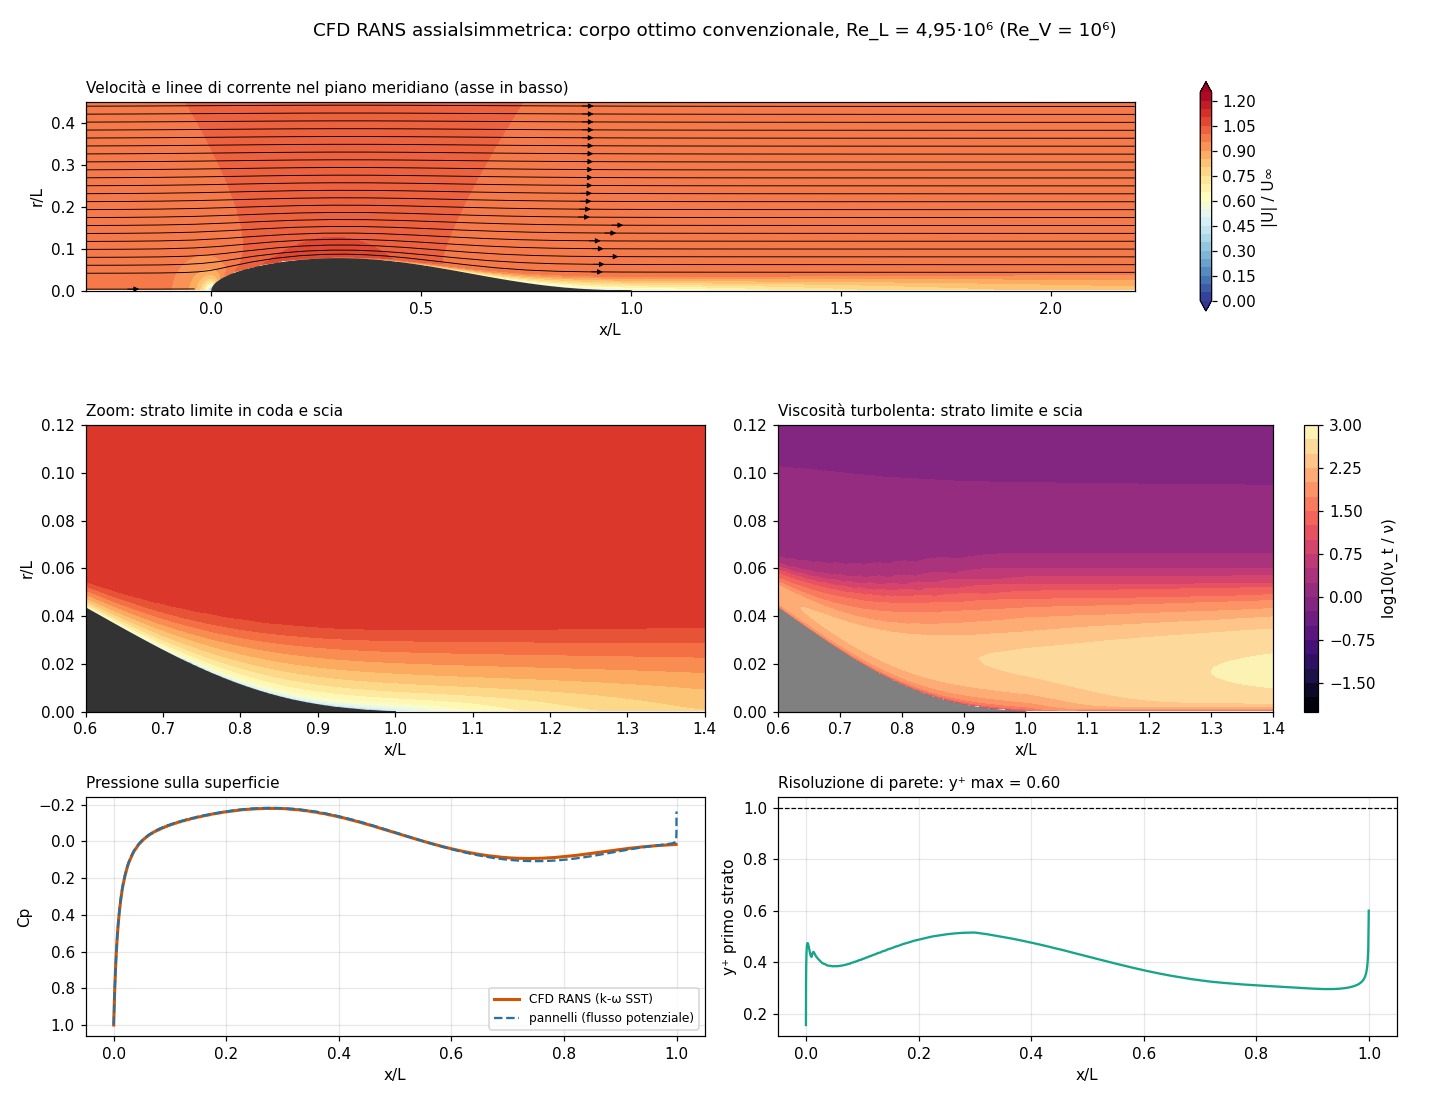
\includegraphics[width=0.8\linewidth]{cfd_conv_1e6f.png}
\caption{RANS versus reduced-order model, bare body at $\ReV=10^6$.}\label{fig:cfdconv}
\end{figure}
\begin{figure}[p]\centering
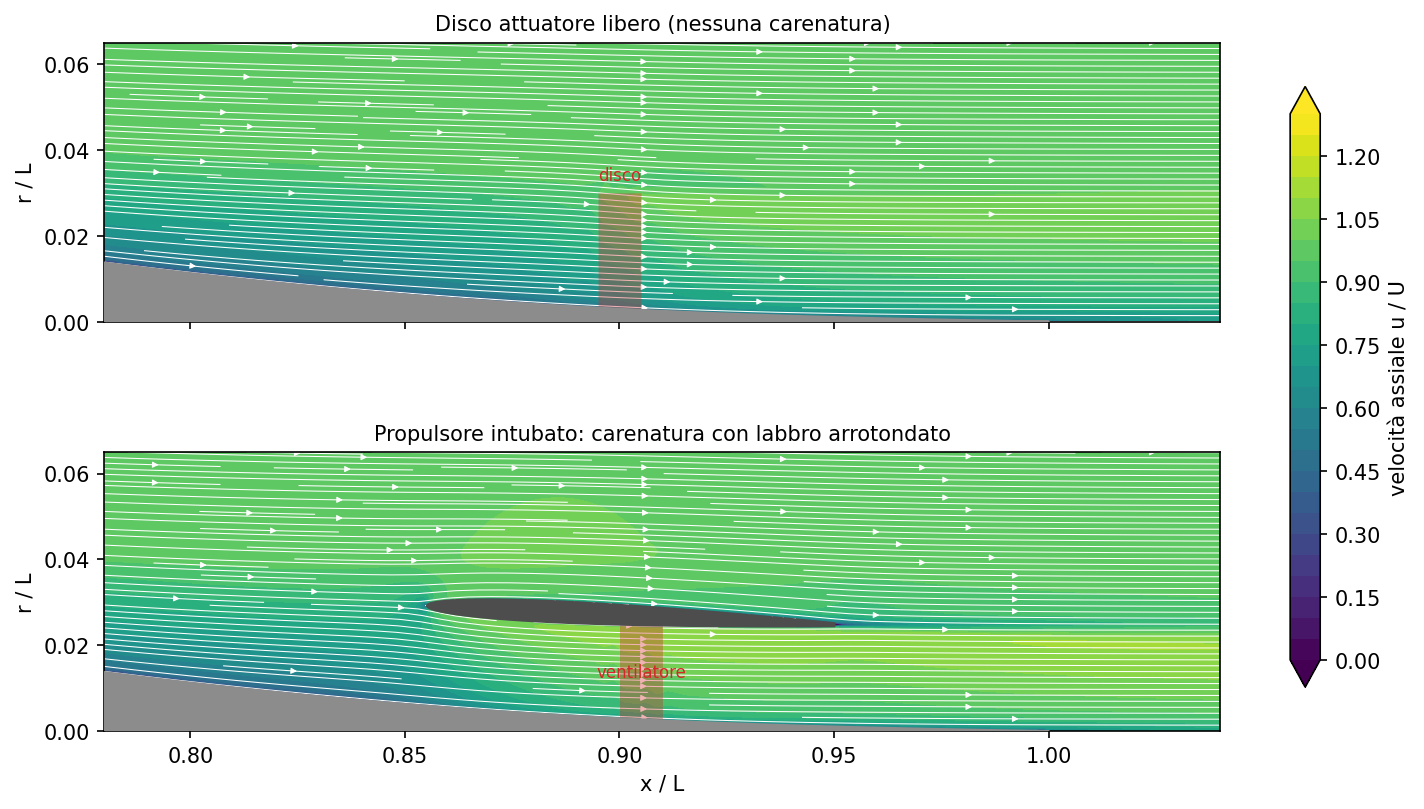
\includegraphics[width=0.8\linewidth]{carena_flusso.png}
\caption{Flow near the tail with the ducted intake (case D).}\label{fig:carena}
\end{figure}

\begin{thebibliography}{9}
\bibitem{hoerner1965} S.~F. Hoerner, \emph{Fluid-Dynamic Drag}, published by the author, 1965.
\bibitem{goldschmied1966} F.~R. Goldschmied, Integrated hull design, boundary-layer
control, and propulsion of submerged bodies, AIAA 2nd Propulsion Joint Specialist Conference,
1966; \emph{J. Hydronautics} 1(1), 1967. \todo{check page numbers}
\bibitem{roepke2012} J.~Roepke, \emph{An experimental investigation of a Goldschmied
propulsor}, MSc thesis, California Polytechnic State University, San Luis Obispo, 2012.
\bibitem{smith1993} L.~H. Smith, Wake ingestion propulsion benefit, \emph{J. Propulsion and
Power} 9(1), 1993.
\bibitem{drela2009} M.~Drela, Power balance in aerodynamic flows, \emph{AIAA J.} 47(7), 2009.
\bibitem{dellacorte2022} B.~Della~Corte, M.~van~Sluis, L.~L.~M. Veldhuis, A.~Gangoli~Rao,
Power balance analysis experiments on an axisymmetric fuselage with an integrated
boundary-layer-ingesting fan, \emph{AIAA J.}, doi:10.2514/1.J060570.
\bibitem{menter1994} F.~R. Menter, Two-equation eddy-viscosity turbulence models for
engineering applications, \emph{AIAA J.} 32(8), 1994.
\bibitem{langtry2009} R.~B. Langtry, F.~R. Menter, Correlation-based transition modeling
for unstructured parallelized CFD codes, \emph{AIAA J.} 47(12), 2009.
\end{thebibliography}
\end{document}
